\documentclass[aspectratio=169]{beamer}
\usetheme{simple}
\usepackage[english]{babel}
\usepackage[utf8]{inputenc} 
\usepackage{lmodern}
\usepackage{ragged2e}
\usefonttheme[onlymath]{serif} 
\usepackage[scale=2]{ccicons} 
% \setbeamertemplate{caption}[numbered]
\usepackage{copyrightbox}

\usepackage{graphicx,hyperref,url,pgfplots}
\usepackage{amsmath} 
\usepackage{array,booktabs}
\pgfplotsset{compat=1.13}
\usepackage{bibentry}
\usepackage[alf,abnt-etal-list=0,abnt-etal-cite=2]{abntex2cite}
\usepackage[normalem]{ulem}

\usepackage[
    type={CC},
    modifier={by-nc-sa},
    version={4.0},
]{doclicense}

\setbeamercovered{invisible} 
% \newcommand{\pausar}{\pause}
\newcommand{\pausar}{\pause}
\newcommand{\df}[1]{\,\mathrm{d}#1}
\newcommand{\parcial}[3]{\dfrac{\partial^{#1}#2}{\partial #3^{#1}}}
\newcommand{\cpright}[2]{\copyrightbox[b]{#1}{\tiny Source: #2}}

\usepackage{tikz}
\usetikzlibrary{automata,positioning}
\usepackage{xcolor}
\usetikzlibrary{scopes}
\usepackage{verbatim}
\usetikzlibrary{patterns}

\usepackage{listings}
  \lstdefinestyle{ascii-tree}{
    literate={├}{|}1 {─}{--}1 {└}{+}1 
  }
	\definecolor{codegreen}{rgb}{0,0.6,0}
	\definecolor{codegray}{rgb}{0.5,0.5,0.5}
	\definecolor{codepurple}{rgb}{0.58,0,0.82}
	\definecolor{backcolour}{rgb}{0.92,0.92,0.92}
	\lstset{language=Python, 
	backgroundcolor=\color{backcolour},   
	commentstyle=\color{codegreen},
	keywordstyle=\color{magenta},
	numberstyle=\tiny\color{codegray},
	stringstyle=\color{codepurple},
	basicstyle=\fontsize{8}{11}\ttfamily,
	frame=lines,
%	numbers=left,
	tabsize=2,
	morekeywords={models, lambda, forms},
	showstringspaces=false}


% --------------------------------------------------------------------------------------------

\title{Mobile Robots}
\subtitle{Quaternions}
\date{\today}
\author[Jeferson José de Lima]{
  \textbf{Professor}: Jeferson José de Lima}
\institute{Academic Department of Informatics (DAINF) \\ Federal University of Technology - Paraná (UTFPR) at Pato Branco, PR, Brazil}

\begin{document}
\maketitle
\justify


\begin{frame}{Useful Information}

	\begin{block}{License}
        \doclicenseThis
    \end{block}

	\begin{block}{links:}
		\begin{enumerate}
			\item \href{https://moodle.utfpr.edu.br/course/view.php?id=14218}{Moodle}
			\item \href{https://gitlab.com/cursoseaulas/robotica-movel/-/wikis/home}{Mobile Robots - Gitlab Page}
			\item \href{http://www.rsl.ethz.ch/education-students/lectures/ros.html}{ETH Programming for Robotics - ROS}
		\end{enumerate}
	\end{block}
\end{frame}


\begin{frame}{Quaternions}
	\framesubtitle{What is a quaternion?}
    \begin{itemize}
        \item What is a quaternion
        \item Representing rotation
        \item Geometric view
        \item Transformations to other representations
        \item Topological and metric properties
        \end{itemize}

\end{frame}


\begin{frame}{Quaternions}
	\framesubtitle{Why can't we invert vectors in $\mathbf{R}^3$?}

    \begin{itemize}
        \item We can invert reals.  $x \times \displaystyle\frac{1}{x} = 1$.
        \item We can invert elements of $\mathbf{R}^2$ using complex numbers.
        \item $z \times  \displaystyle\frac{z^*}{|z|^2} = 1$, where $^*$ is complex conjugate.
        \item Can we invert $\mathbf{v} \in \mathbf{R}^3$? \textcolor{red}{No}
        \item How about $\mathbf{v} \in \mathbf{R}^4$? \textcolor{blue}{Yes!}
        \item Hamilton's quaternions are to $\mathbf{R}^3$ what complex numbers are to $\mathbf{R}$.
    \end{itemize}

\end{frame}

\begin{frame}{Quaternions}
	\framesubtitle{Complex numbers versus quaternions}

    \begin{itemize}
    \item To define complex numbers  \cite{jeffcourse_2007}:
    \begin{itemize}
        \item Basis elements $1$ and $i$;
        \item Vector space over reals:  elements have the form $x+i y$;
        \item One more axiom required:  $i^2$ = -1.
    \end{itemize}
    \item To define quaternions:
    \begin{itemize}
        \item Basis elements $1$, $i$, $j$, $k$;
        \item Vector space over reals:  elements have the form $q_0 + q_1 i + q_2 j + q_3 k$;
        \item Six more axioms:
        \begin{align*}
        i^2 &= j^2 = k^2 = -1 \\
        ij &= k \\
        jk &= i \\
        ki &= j
        \end{align*}
    \end{itemize}
\end{itemize}
\end{frame}

\begin{frame}{Quaternions}
	\framesubtitle{Quaternion notation}

    We can write a quaternion several ways:
    \begin{align*}
        q &= q_0 + q_1 i + q_2 j + q_3 k\\
        q &= (q_0, q_1, q_2, q_3)\\
        q &= q_0 + \mathbf{q}
    \end{align*}
    where $q_0$ is the \emph{scalar part} and $\mathbf{q}$ is the \emph{vector part}
\end{frame}


\begin{frame}{Quaternions}
	\framesubtitle{Quaternion product}

    We can write a quaternion product several ways:
    \begin{align*}
      pq &= (p_0 + p_1 i + p_2 j + p_3 k)  (q_0 + q_1 i + q_2 j + q_3 k)\\
            &= (p_0 q_0 - p_1 q_1 - p_2 q_2 - p_3 q_3) + \ldots i + \ldots j + \ldots k \\
      pq &= (p_0 + \mathbf{p}) (q_0 + \mathbf{q}) \\
            &= (p_0 q_0 + p_0 \mathbf{q} + q_0 \mathbf{p} + \mathbf{p} \mathbf{q})
    \end{align*}
    So what is $\mathbf{p} \mathbf{q}$?  Cross product?  Dot product?
    
    Both!  Cross product minus dot product!
    
    \begin{equation}
        pq = (p_0 q_0 - \mathbf{p} \cdot \mathbf{q} + p_0 \mathbf{q} + q_0 \mathbf{p} + \mathbf{p} \times \mathbf{q}) 
    \end{equation}

\end{frame}




\begin{frame}{Quaternions}
	\framesubtitle{Conjugate, length}

    \begin{itemize}
        \item Quaternion \textbf{conjugate}:
        \begin{equation}
        q^* = q_0 - q_1 i - q_2 j - q_3 k
        \end{equation}
        \item Note that
        \begin{align*}
        q q^* &= (q_0 + \mathbf{q})(q_0 - \mathbf{q}) \\
                    &= q_0^2 + q_0 \mathbf{q} - q_0 \mathbf{q} - \mathbf{q} \mathbf{q}  \\
                    &= q_0^2 + \mathbf{q} \cdot \mathbf{q} - \mathbf{q} \times \mathbf{q}  \\
                    &= q_0^2 + q_1^2 + q_2^2 + q_3^2
        \end{align*}
        \item Quaternion \textbf{length}:
        \begin{equation}
            |q| = \sqrt{q q^*} = \sqrt{q_0^2 + q_1^2 + q_2^2 + q_3^2} 
        \end{equation}
    \end{itemize}
\end{frame}


\begin{frame}{Quaternions}
	\framesubtitle{Quaternion inverse}
    \begin{itemize}
        \item[]Note that every quaternion other than the additive identity $0$ has an inverse:
        \[ q^{-1} = \frac{q^*}{|q|^2} \]
    \end{itemize}
        That means quaternions are a linear algebra and a field.  Hamilton's dream.  Quaternions are the only extension of  complex numbers that is both a linear algebra and a field.  If 1D numbers are the reals, and 2D numbers are the complex numbers, then 4D numbers are quaternions, and that's all there is.  (Frobenius?)
    \end{frame}

\begin{frame}{Quaternions}
    \framesubtitle{Rotation using unit quaternions}

    \begin{itemize}
        \item Let $q$ be a unit quaternion, i.e. $|q|=1$.
        \begin{itemize}
        \item  It can be expressed as
        \begin{equation}
            q = \cos \frac{\theta}{2} + \sin \frac{\theta}{2} \hat{\mathbf{n}} 
        \end{equation}
        \end{itemize}
        \item Let $x = 0 + \mathbf{x}$ be a "pure vector".
        \item Let $x^\prime = qxq^*$.
        \item Then $x^\prime$ is the pure vector $\operatorname(\theta,\hat{\mathbf{n}}) \mathbf{x}$!!!
    \end{itemize}

\end{frame}


\begin{frame}{Quaternions}
    \framesubtitle{Proof that unit quaternions work}
    \begin{itemize}
        \item[] Expand the product $qxq^*$;
        \item[] Apply half angle formulas;
        \item[] Simplify;
        \item[] to obtain Rodrigues's formula.
    \end{itemize}
\end{frame}


\begin{frame}{Quaternions}
    \framesubtitle{Why $\theta / 2$?  Why $qxq^*$ instead of $qx$?}

    Two puzzling things.  In analogy with complex numbers, why not use
    \begin{align*} 
           p &= \cos\theta + \hat{\mathbf{n}}\sin\theta \\
           \mathbf{x}^\prime &= p\mathbf{x}
    \end{align*}
    To explore that idea, define a map $L_p(q) = pq$ with $p$ a unit pure vector.
    Note that $L_p(q)$ can be written:
    \begin{equation*}
            L_p(q) = \left(\begin{array}{cccc}
                             p_0 & -p_1 & -p_2 & -p_3 \\
                             p_1 &  p_0 & -p_3 &  p_2 \\
                             p_2 &  p_3 &  p_0 & -p_1 \\
                             p_3 & -p_2 &  p_1 &  p_0 \\
                     \end{array}\right)
                     \left(\begin{array}{c}
                            q_0 \\ q_1 \\ q_2 \\ q_3 \\
                     \end{array}\right)
    \end{equation*}
    Note that the matrix above is orthonormal.  $L_p$ is a rotation of
    Euclidean 4 space!
    (Without even using the fact that $p$ is a pure vector.)
\end{frame}


\begin{frame}{Quaternions}
    \framesubtitle{Why $\theta / 2$?  Why $qxq^*$ instead of $qx$?}
    \emph{not} a rotation of the 3D subspace of pure vectors.  Some of
    the 3D subspace leaks into the fourth dimension.

    Consider an example using $p = i$.  Is it a rotation about $i$ of $\pi/2$?
    \begin{figure}[h!]
    \centerline{
    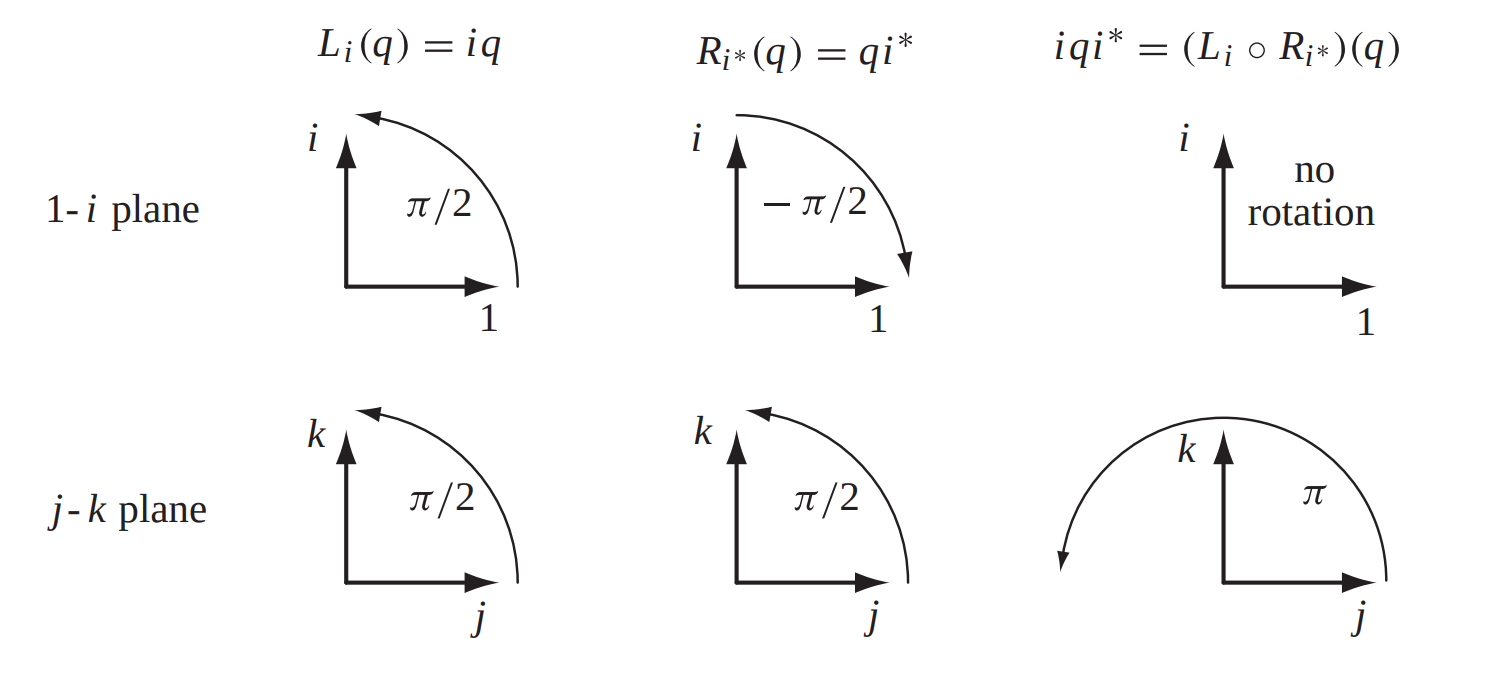
\includegraphics[height = 5cm]{images/quatrot.png}}
    \end{figure}
\end{frame}


\begin{frame}{Quaternions}
    \framesubtitle{What do we do with a representation?}
    Rotate a point:  $qxq^*$.

    Compose two rotations:
    \begin{equation}
        q(p\mathbf{x} p^*)q^* = (qp)\mathbf{x}(qp)^*
    \end{equation}

    Convert to other representations:
    \begin{itemize}
        \item  From axis-angle to quaternion:
        \begin{equation}
            q = \cos \frac{\theta}{2} + \sin \frac{\theta}{2} \hat{\mathbf{n}}
        \end{equation}

        \item  From quaternion to axis-angle:
        \begin{align*}
            \theta &= 2 \tan^{-1}(|{\mathbf{q}}|, q_0) \\
            \hat{\mathbf{n}} &= {\mathbf{q}}/|{\mathbf{q}}|
        \end{align*}
        assuming $\theta$ is nonzero. 
    \end{itemize}
\end{frame}


\begin{frame}{Quaternions}
    \framesubtitle{From quaternion to rotation matrix}

        Just expand the product
        \begin{equation}
        qxq^* = 
        \left( \begin{array}{ccc}
                q_0^2 + q_1^2 - q_2^2 - q_3^2 
                        & 2(q_1 q_2 - q_0 q_3) 
                        & 2(q_1 q_3 + q_0 q_2) \\
                2(q_1 q_2 + q_0 q_3) 
                        & q_0^2 - q_1^2 + q_2^2 - q_3^2 
                        & 2 (q_2 q_3 - q_0 q_1) \\
                2(q_1 q_3 - q_0 q_2) 
                        & 2 (q_2 q_3 + q_0 q_1)
                        & q_0^2 - q_1^2 - q_2^2 + q_3^2 \\
                        \end{array}\right) \mathbf{x}
        \end{equation}
\end{frame}



\begin{frame}{Quaternions}
    \framesubtitle{From rotation matrix to quaternion}

    \begin{itemize}
        \item Given $R = (r_{ij})$, solve expression on previous page for
        quaternion elements $q_i$ 
        \item Linear combinations of diagonal elements seem to solve the problem:
        \begin{align*}
                q_0^2 =& \frac{1}{4} (1 + r_{11} + r_{22} + r_{33}) \\
                q_1^2 =& \frac{1}{4} (1 + r_{11} - r_{22} - r_{33}) \\
                q_2^2 =& \frac{1}{4} (1 - r_{11} + r_{22} - r_{33}) \\
                q_3^2 =& \frac{1}{4} (1 - r_{11} - r_{22} + r_{33})   
        \end{align*}
        
        so take four square roots and you're done?  You have to figure the
        signs out.  There is a better way $\ldots$
    \end{itemize}

\end{frame}

\begin{frame}{Quaternions}
    \framesubtitle{Look at the off-diagonal elements}
\begin{itemize}
    \item[]
    \begin{align*}
            q_0 q_1 =& \frac{1}{4}(r_{32} - r_{23}) \\
            q_0 q_2 =& \frac{1}{4}(r_{13} - r_{31}) \\
            q_0 q_3 =& \frac{1}{4}(r_{21} - r_{12}) \\
            q_1 q_2 =& \frac{1}{4}(r_{12} + r_{21}) \\
            q_1 q_3 =& \frac{1}{4}(r_{13} + r_{31}) \\
            q_2 q_3 =& \frac{1}{4}(r_{23} + r_{32})
    \end{align*}
    
    \item[]  Given any one $q_i$, could solve the above for the other three.
    \end{itemize}
\end{frame}



\begin{frame}{Quaternions}
    \framesubtitle{Exercice}

\end{frame}


\begin{frame}[t, allowframebreaks]
	\frametitle{Referências}
	\bibliography{../references.bib}
\end{frame}

\end{document}